
\lecture{Examples of the Normal Distribution}{normal-distributions-examples}
\section{Examples of the Normal Distribution}

\title{Examples of the Normal Distribution}
\subtitle{Moar Normal!}

%\author{Kelly Black}
%\institute{Clarkson University}
\date{30 January 2015}

\begin{frame}
  \titlepage
\end{frame}

\begin{frame}
  \frametitle{Outline}
  \tableofcontents[hideothersubsections,sectionstyle=show/hide]
\end{frame}


\subsection{Clicker Quiz}


\iftoggle{clicker}{%
  \begin{frame}{Clicker Quiz}

    What is the probability that a normally distributed random
    variable that follows a standard normal will be less than -0.45?

    \vfill

    \begin{tabular}{l@{\hspace{3em}}l@{\hspace{3em}}l}
      A:  .3264  & B: .3632  & C: .6736
    \end{tabular}

    \vfill
    \vfill
    \vfill

  \end{frame}
}


\subsection{Examples}

\begin{frame}
  \frametitle{Example}

  You are examining a portfolio of stocks. The total change in the
  value of an individual stock is normally distributed with a mean of
  0.5 and a standard deviation of 4.4. You want to decide which ones
  are in the top 25\% in gains based solely on the price change. What
  is the cut off?

  \vfill

  \only<2->{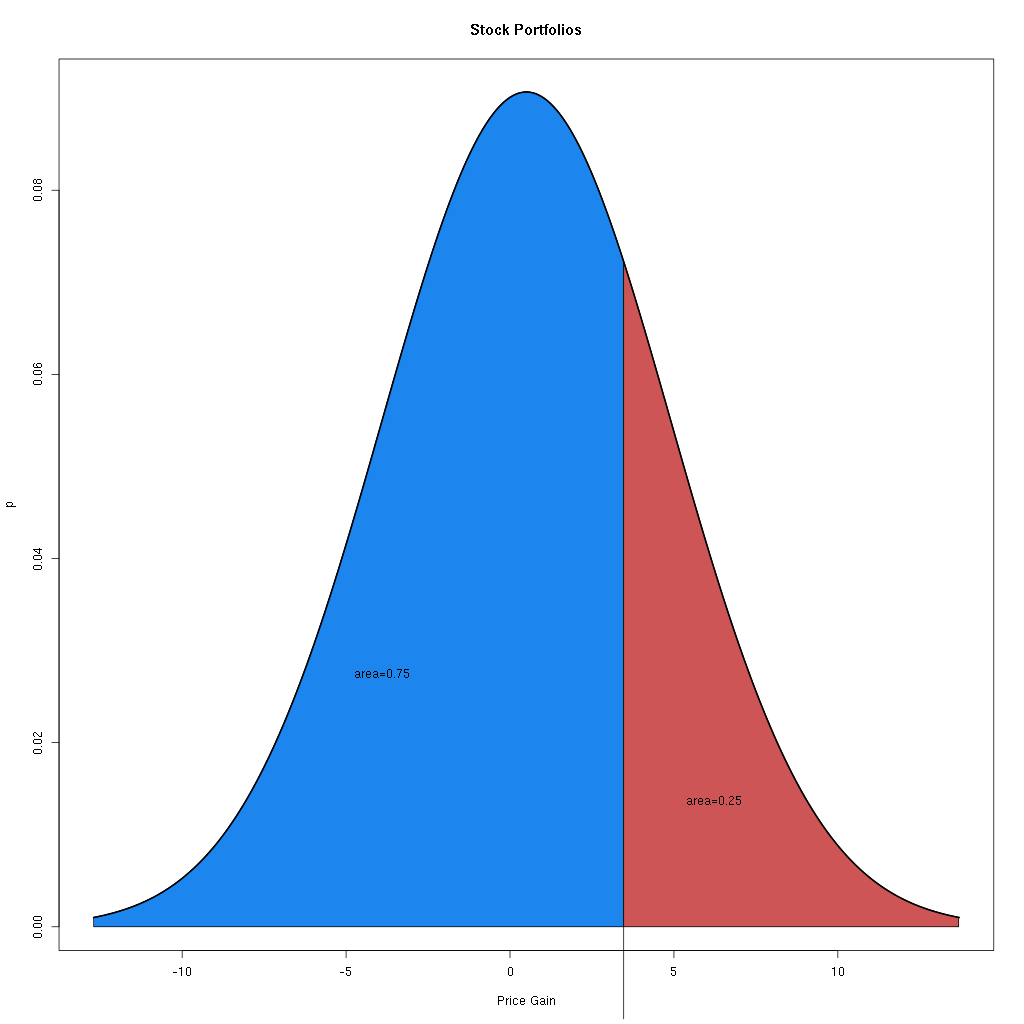
\includegraphics[width=12em]{img/topStockPicks}}

  \vfill


  \only<3->{ans: 3.45}
\end{frame}





\begin{frame}
  \frametitle{Example}

  A normally distributed random variable has a mean of 3.0 and a
  standard deviation of 4.5. If I take one sample what is the
  probability that it is less than zero?

  \vfill

  \only<2->{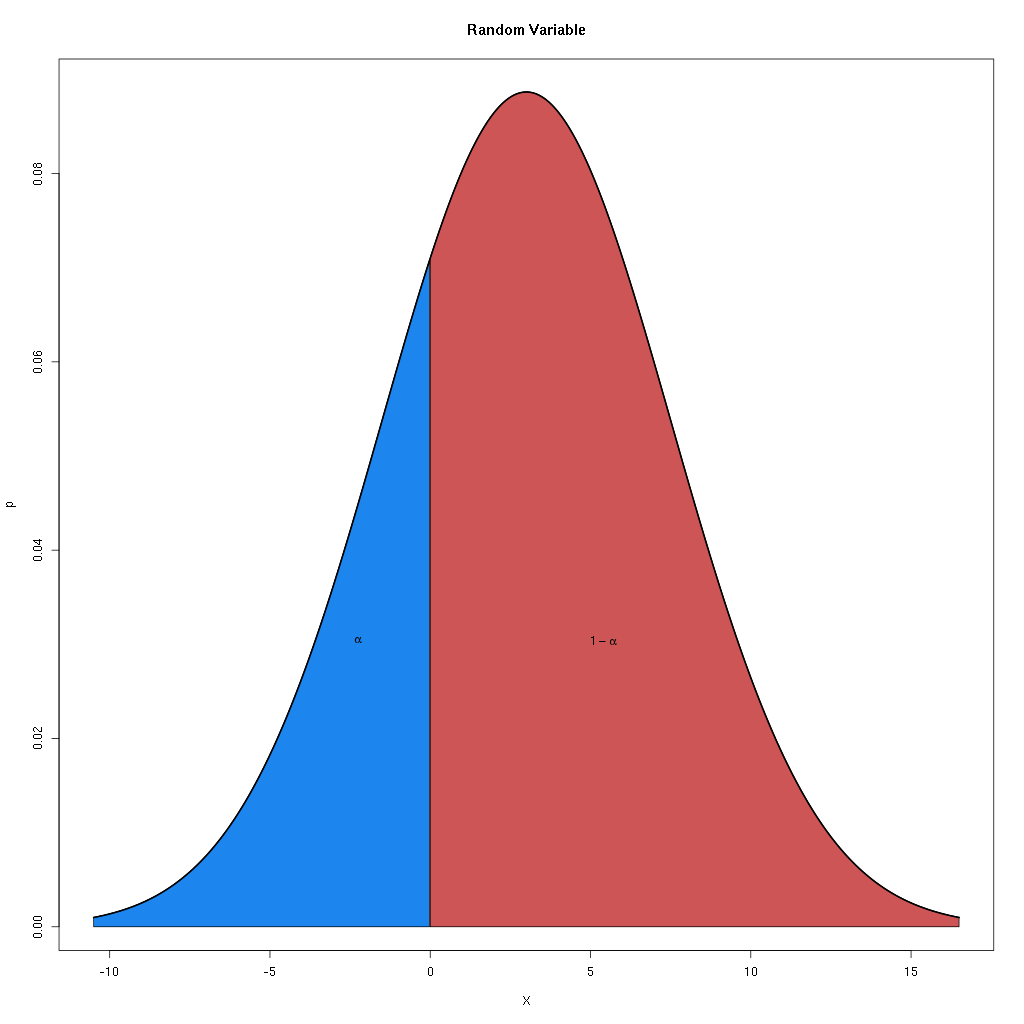
\includegraphics[width=12em]{img/normalRVMean3}}

  \vfill

  \only<3->{ans: 0.2514}

%  \only<2->
%  {
%    If I take four samples what is the probability that it is less
%    than zero?
%  }
%
%  \vfill

\end{frame}

\iftoggle{clicker}{%
  \begin{frame}
    \frametitle{Clicker Quiz - Starting Salaries}

    The mean starting salaries for business majors is approximately
    normally distributed with a mean of \$56,000 and a standard
    deviation of \$5,000. What is the probability that a single,
    randomly chosen business major will have an offer of more than
    \$63,000 per year?

    \vfill

    \begin{tabular}{l@{\hspace{3em}}l@{\hspace{3em}}l}
      A:  0.0808  & B: 0.919  & C: 1.4
    \end{tabular}

    \vfill
    \vfill
    \vfill



  \end{frame}
}





\iftoggle{clicker}{%
  \begin{frame}
    \frametitle{Clicker Quiz}

    The total change in a stock's price on one particular day is
    approximately normally distributed and has a mean of -.35\$ with a
    standard deviation of .86\$.  What is the probability that the
    price change in a randomly chosen stock will be more than zero?

    \vfill

    \begin{tabular}{l@{\hspace{3em}}l@{\hspace{3em}}l@{\hspace{3em}}l}
      A: 0.0516  & B: 0.3409 & C: 0.6580 & D: 0.9484
    \end{tabular}

    \vfill
    \vfill
    \vfill

  \end{frame}
}


\begin{frame}
  \frametitle{Example}

  A normally distributed random variable has a mean of 12.0, and the
  probability that it is less than 8.0 is approximately 0.25. What is
  the standard deviation?

  \vfill

  \only<2->{ans: 5.97}
\end{frame}


\begin{frame}
  \frametitle{Example}

  A normally distributed random variable has a mean of -2.0 and a
  standard deviation of 5.0. Find the value, $x$, so that there is a
  probability of 0.30 that the random variable is bigger than than
  $x$.

  \vfill

  \only<2->{ans: 0.6}
\end{frame}


\begin{frame}{If Time: Example}

  The waiting times for patients at a doctor's office is normally
  distributed with a mean of 8.4 minutes and a standard deviation of
  2.1 minutes. What is the waiting time for which 5\% of the patients
  must wait longer?
  
  \vfill

  \only<2->{11.8 minutes}
\end{frame}


\begin{frame}{If Time: Example}

  A dynamometer is used to measure a patient's elbow flexion
  strength. In the article \textit{The Influence of Age and Type of
    Force on Muscle Strength Capabilities in Women}, Tokarski
  \textit{et al}, International Journal of Occupational Safety and
  Ergonomics (JOSE) 2012, Vol. 18, No. 1, 47–57 it is estimated that
  the mean elbow flexion strength for the right arm of women between
  20 and 25 years old is 62N with a standard deviation of 18N. A
  woman between the age of 20 and 25 is chosen at random. What is the
  probability that her right arm's elbow flexion strength is greater
  than 85N?

  
  \vfill

  \only<2->{0.1003}
\end{frame}


\begin{frame}{If Time: Example}

  A dynamometer is used to measure a patient's elbow flexion
  strength. In the article \textit{The Influence of Age and Type of
    Force on Muscle Strength Capabilities in Women}, Tokarski
  \textit{et al}, International Journal of Occupational Safety and
  Ergonomics (JOSE) 2012, Vol. 18, No. 1, 47–57 it is estimated that
  the mean elbow flexion strength for the right arm of women between
  40 and 45 years old is 40N with a standard deviation of 17N. A
  woman between the age of 40 and 45 is chosen at random. What is the
  probability that her right arm's elbow flexion strength is greater
  than 85N?

  
  \vfill

  \only<2->{0.0040}
\end{frame}



% LocalWords:  Clarkson pausesection hideallsubsections hideothersubsections
% LocalWords:  sectionstyle
